\documentclass[11pt]{report}

% Paquetes y configuraciones adicionales
\usepackage{graphicx}
\usepackage[export]{adjustbox}
\usepackage{caption}
\usepackage{float}
\usepackage{titlesec}
\usepackage{geometry}
\usepackage[hidelinks]{hyperref}
\usepackage{titling}
\usepackage{titlesec}
\usepackage{parskip}
\usepackage{wasysym}
\usepackage{tikzsymbols}
\usepackage{fancyvrb}
\usepackage[spanish]{babel}

\newcommand{\subtitle}[1]{
  \posttitle{
    \par\end{center}
    \begin{center}\large#1\end{center}
    \vskip0.5em}
}

% Configura los márgenes
\geometry{
    left=2cm,   % Ajusta este valor al margen izquierdo deseado
    right=2cm,  % Ajusta este valor al margen derecho deseado
    top=3cm,
    bottom=3cm,
}

% Configuración de los títulos de las secciones
\titlespacing{\section}{0pt}{\parskip}{\parskip}
\titlespacing{\subsection}{0pt}{\parskip}{\parskip}
\titlespacing{\subsubsection}{0pt}{\parskip}{\parskip}

% Redefinir el formato de los capítulos y añadir un punto después del número
\makeatletter
\renewcommand{\@makechapterhead}[1]{%
  \vspace*{0\p@} % Ajusta este valor para el espaciado deseado antes del título del capítulo
  {\parindent \z@ \raggedright \normalfont
    \ifnum \c@secnumdepth >\m@ne
        \huge\bfseries \thechapter.\ % Añade un punto después del número
    \fi
    \interlinepenalty\@M
    #1\par\nobreak
    \vspace{10pt} % Ajusta este valor para el espacio deseado después del título del capítulo
  }}
\makeatother

% Configura para que cada \chapter no comience en una pagina nueva
\makeatletter
\renewcommand\chapter{\@startsection{chapter}{0}{\z@}%
    {-3.5ex \@plus -1ex \@minus -.2ex}%
    {2.3ex \@plus.2ex}%
    {\normalfont\Large\bfseries}}
\makeatother

\begin{document}

% Portada del informe
\title{Seguridad e inyección en SQL}
\subtitle{Administración y Diseño de Bases de Datos}
\author{Cheuk Kelly Ng Pante, Javier González de la Barreda Arimany y Samuel Toledo Hernández}
\date{\today}

\maketitle

\pagestyle{empty} % Desactiva la numeración de página para el índice

% Índice
\tableofcontents

% Nueva página
\cleardoublepage

\pagestyle{plain} % Vuelve a activar la numeración de página
\setcounter{page}{1} % Reinicia el contador de página a 1
% Secciones del informe
% Capitulo 
\chapter{Introducción a ciberseguridad}
La ciberseguridad es la práctica de proteger equipos, redes, aplicaciones de software, sistemas críticos y
datos de posibles amenazas digitales. Las organizaciones tienen la responsabilidad de proteger los datos para
mantener la confianza del cliente y cumplir la normativa. Utilizan medidas y herramientas de ciberseguridad
para proteger los datos confidenciales del acceso no autorizado, así como para evitar interrupciones en las
operaciones empresariales debido a una actividad de red no deseada. Las organizaciones implementan la ciberseguridad 
al optimizar la defensa digital entre las personas, los procesos y las tecnologías. 

\section{¿Por qué es importante la ciberseguridad?}
Igual que protegen los recursos físicos, deben proteger también los recursos digitales y los sistemas frente al acceso no intencionado. El evento no intencionado de incumplimiento
y acceso no autorizado a un sistema informático, una red o recursos conectados se denomina ciberataque. El éxito de
un ciberataque produce la exposición, sustracción, eliminación o alteración de datos confidenciales. Las medidas de
ciberseguridad defienden frente a ciberataques y proporcionan los siguientes beneficios:

\begin{itemize}
  \item \textbf{Prevención o reducción del costo de las brechas} \\
  Las organizaciones que implementan estrategias de ciberseguridad minimizan las consecuencias no deseadas de ciberataques
  que pueden afectar a la reputación empresarial, las capacidades financieras, las operaciones empresariales y la confianza
  del cliente. Por ejemplo, las compañías activan planes de recuperación de desastres para contener las posibles intrusiones
  y minimizar las interrupciones en las operaciones empresariales.

  \item \textbf{Mantener una conformidad normativa} \\
  Las empresas de sectores y regiones específicos deben cumplir con los requisitos normativos para proteger los datos confidenciales
  frente a posibles riesgos cibernéticos. Por ejemplo, las empresas que operan en Europa deben cumplir el Reglamento General de Protección de Datos (GDPR),
  que espera que las organizaciones adopten las medidas de ciberseguridad adecuadas para garantizar la privacidad de los datos. 

  \item \textbf{Mitigación de las ciberamenazas} \\
  Los ciberataques evolucionan a la par que las tecnologías cambiantes. Los delincuentes utilizan nuevas herramientas y elaboran nuevas estrategias para el acceso 
  no autorizado al sistema. Las organizaciones emplean y actualizan las medidas de ciberseguridad para mantenerse al día de estas tecnologías y herramientas de ataque
  digital nuevas y en desarrollo. 
\end{itemize}

\section{Los ataques más comunes contra la ciberseguridad}
Algunos de los tipos de ataques más comunes contra la ciberseguridad son los siguientes:
\begin{itemize}
  \item \textbf{Malware:} Significa software malintencionado. Incluye una variedad de programas de software creados para permitir que terceras partes accedan de manera no autorizada a información confidencial o interrumpan el funcionamiento normal de una infraestructura crítica. Entre los ejemplos más comunes de malware se incluyen los troyanos, spyware y virus.

  \item \textbf{Ransomware:} Hace referencia a un modelo empresarial y a un amplio rango de tecnologías asociadas que los delincuentes pueden usar para extorsionar dinero a entidades.
  
  % Nueva página
  \cleardoublepage

  \item \textbf{Phishing: } Es una ciberamenaza que usa técnicas de ingeniería social para engañar a los usuarios a fin de que revelen información de identificación personal. Por ejemplo, los atacantes cibernéticos envían correos electrónicos que inducen a los usuarios a hacer clic e introducir los datos de la tarjeta de crédito en una página web de pagos ficticia. 
  Los ataques de pishing también pueden incitar a la descarga de datos adjuntos malintencionados que instalen malware en los dispositivos de la empresa.

  \item \textbf{DDoS: } Es un trabajo coordinado para sobrecargar un servidor enviando un gran volumen de solicitudes falsas. Estos eventos impiden que los usuarios normales se conecten o accedan al servidor de destino. 
  
  \item \textbf{Amenaza interna: } Es un riesgo de seguridad introducido por personal con malas intenciones dentro de una organización. El personal posee acceso de alto nivel a los sistemas informáticos y puede desestabilizar la seguridad de la infraestructura desde dentro. 
\end{itemize}

\section{Funcionamiento de la ciberseguridad}

Las organizaciones recurren a la contratación de especialistas en ciberseguridad para llevar a cabo la implementación de estrategias destinadas a salvaguardar sus sistemas informáticos, redes, almacenamiento de datos, aplicaciones y demás dispositivos conectados. Estos profesionales, a su vez, evalúan los riesgos de seguridad presentes en dichos elementos.

Posteriormente, se encargan de desarrollar un marco integral de ciberseguridad y de poner en marcha medidas de protección dentro de la organización. Un programa exitoso en esta área implica la capacitación de los empleados en prácticas de seguridad recomendadas, así como el uso automatizado de tecnologías de defensa cibernética para fortalecer la infraestructura de tecnologías de la información ya existente.

Estos componentes trabajan de manera conjunta para establecer diversas capas de protección en todos los puntos de acceso a los datos, abordando amenazas potenciales. Además, se dedican a la identificación de riesgos, la protección de identidades, infraestructuras y datos, la detección de anomalías y eventos, la respuesta y el análisis de la causa raíz, así como la ejecución de procesos de recuperación tras un incidente.




% Nueva página
\cleardoublepage

% Capitulo 1
\chapter{Introducción a la seguridad de bases de datos}
\section{Introducción a las bases de datos}
Una base de datos consiste en una colección de datos interrelacionados que representan
información sobre una organización o área en particular. Estas bases de datos están
organizadas según modelos de datos que definen la estructura, almacenamiento y
manipulación de la información. El modelo principal es un modelo relacional que representa
datos a través de tablas y crea relaciones entre ellos.

Los sistemas de gestión de bases de datos (DBMS) son programas informáticos que
gestionan, modifican, consultan y crean bases de datos. Entre sus ventajas importantes se
incluyen la independencia de los datos con respecto a la aplicación respectiva, la garantía
de integridad mediante reglas de validación; seguridad de la información mediante control
de acceso; y optimización del rendimiento a través de índices/vistas.

En el diseño de bases de datos intervienen una variedad de etapas, incluido el análisis de
requisitos, el diseño conceptual, el diseño lógico y el diseño físico. Los modelos de entidad,
atributos y relaciones se utilizan en el modelo de relación de entidad para representar datos
en el diseño conceptual. El modelo relacional es la base del diseño lógico, ya que presenta
datos a través de tablas, claves y restricciones.

El lenguaje utilizado para consultar la base de datos es un conjunto de instrucciones que
permiten a los usuarios seleccionar, insertar, actualizar y eliminar datos. La mayoría de los
DBMS pueden ser compatibles con SQL, qué es el lenguaje de consulta más utilizado.

En el ámbito de la programación de bases de datos, se emplean subrutinas, que son
bloques de código encargados de llevar a cabo tareas específicas relacionadas con los
datos. Estas subrutinas pueden manifestarse como procedimientos almacenados o
funciones, diferenciándose en que los procedimientos almacenados pueden retornar varios
valores o ninguno, mientras que las funciones solo pueden devolver un valor. La ejecución
de estas subrutinas dentro del Sistema de Gestión de Bases de Datos (SGBD) contribuye a
mejorar tanto la eficiencia como la seguridad de las bases de datos

\section{Seguridad de bases de datos}
La seguridad de la base de datos abarca un conjunto de herramientas, medidas y controles
diseñados para proteger la integridad, confidencialidad y disponibilidad de los datos
almacenados en una base de datos. Estas “copias” están implementadas para evitar el
acceso no autorizado, modificaciones inapropiadas o pérdidas accidentales. En este
contexto, se cubrirán aspectos técnicos y organizativos, incluidas actividades como
autenticación, auditoría, cumplimiento normativo, gestión de riesgos, educación, etc.

La importancia de la seguridad de las bases de datos reside en su función esencial para
asegurar el funcionamiento adecuado de las organizaciones y la salvaguardia de la
privacidad de las personas. Para preservar la integridad del sistema, resulta crucial hacer
frente a amenazas como ataques internos, errores humanos, vulnerabilidades de software,
ataques de inyección SQL, ataques de denegación de servicio y la presencia de malware.

Ante las amenazas mencionadas, se sugiere adoptar las mejores prácticas de
ciberseguridad, que incluyen medidas como salvaguardar la integridad física, aplicar
controles administrativos y de acceso a la red, asegurar dispositivos y cuentas de usuarios
finales, proteger el software de bases de datos, garantizar la seguridad de servidores de
aplicaciones y web, así como implementar precauciones en las copias de respaldo y llevar a
cabo auditorías periódicas.

La seguridad de las bases de datos emerge como un tema de gran importancia y
complejidad. En este contexto, se busca resguardar la información almacenada en dichas
bases contra accesos no autorizados, alteraciones indebidas y pérdidas accidentales o
maliciosas. La protección de la base de datos involucra diversos elementos críticos como:

\begin{itemize}
\item \textbf{Datos de la base de datos:} Esta información, que abarca desde nombres y
contraseñas hasta números de tarjetas de crédito y debe mantenerse confidencial,
íntegra y accesible únicamente para usuarios autorizados.
\item \textbf{Sistema de gestión de bases de datos (DBMS):} Desempeña un papel fundamental
al crear, administrar y manipular las bases de datos. Es esencial que el DBMS esté
actualizado, configurado y protegido de manera adecuada para prevenir
vulnerabilidades y ataques.
\item \textbf{Aplicaciones asociadas:} Los programas que interactúan con la base de datos para
realizar diversas operaciones deben validar y filtrar las entradas de los usuarios.
Además, es crucial que utilicen consultas parametrizadas o procedimientos
almacenados, y limiten los permisos y privilegios de los usuarios y las bases de
datos.
\item \textbf{Servidor de base de datos físico y/o virtual y hardware subyacente:} Estos
dispositivos, ya sean físicos o virtuales, donde residen la base de datos y el DBMS,
deben contar con protección física, sistemas de copia de seguridad y recuperación,
así como medidas de seguridad de red, como firewalls, antivirus y cifrado.
\item \textbf{Infraestructura informática y/o de red para acceder a la base de datos:} Los medios a
través de los cuales usuarios y aplicaciones se comunican con la base de datos,
como ordenadores, dispositivos móviles e internet, deben garantizar la seguridad y
privacidad de las comunicaciones. Esto implica el uso de protocolos seguros,
contraseñas robustas, certificados de seguridad, entre otras medidas.
\end{itemize}

La importancia de asegurar las bases de datos radica en la necesidad de prevenir o reducir
al mínimo los riesgos y las consecuencias asociadas a los ciberataques. Estos eventos
pueden resultar en daños irreparables tanto para los datos almacenados como para las
organizaciones y los usuarios involucrados. Algunos de los ciberataques más comunes y
peligrosos pueden ser:

\begin{itemize}
\item \textbf{La inyección SQL:} Implica la introducción de código SQL malicioso en las entradas
de los usuarios para alterar o acceder a la información de la base de datos. Este tipo
de ataque puede ocasionar la pérdida o el robo de datos sensibles, la modificación o
eliminación de información crucial, la ejecución de comandos arbitrarios en el
servidor, o la revelación de datos internos o confidenciales de una organización.
\item \textbf{El robo de credenciales:} Se refiere a la obtención de contraseñas o nombres de
usuario de usuarios o aplicaciones que acceden a la base de datos. El propósito de
este ataque es suplantar identidades o llevar a cabo acciones no autorizadas, lo que
puede resultar en acceso no autorizado a los datos, alteración o borrado de
información, o la propagación de malware o virus.
\item \textbf{El ransomware:} Implica cifrar los datos de la base de datos o bloquear su acceso,
con el objetivo de exigir un rescate a cambio de su liberación. Este tipo de ataque
puede conducir a la inaccesibilidad de los datos, interrupciones en el funcionamiento
del negocio o el pago de grandes sumas de dinero
\end{itemize}

La seguridad de las bases de datos exige la implementación de un conjunto integral de
medidas técnicas, organizativas y legales destinadas a resguardar los datos de posibles
amenazas, tanto internas como externas, como hackers, empleados deshonestos, errores
humanos, fallas de hardware o software, desastres naturales y violaciones normativas.
Diversas prácticas, políticas y tecnologías pueden ser adoptadas para fortalecer la
seguridad de las bases de datos, entre las que se encuentran:
\begin{itemize}
  \item Diseñar una arquitectura de base de datos segura que separe los datos sensibles de
  los no sensibles, que minimice los puntos de acceso y que aplique el principio de
  mínimo privilegio.
  \item Implementar un sistema de gestión de bases de datos (DBMS) actualizado y
  configurado adecuadamente, que ofrezca funciones integradas de seguridad, tales
  como cifrado, control de acceso, registro de eventos y detección de anomalías.
  \item Desarrollar una aplicación segura que utilice métodos de conexión seguros, que
  evite la inyección de código malicioso, valide los datos de entrada y cifre la
  información en tránsito y en reposo.
  \item Llevar a cabo pruebas de seguridad periódicas que evalúen la vulnerabilidad de la
  base de datos e identifiquen y corrijan posibles debilidades o brechas.
  \item Impartir formación y concienciación a los usuarios y administradores de la base de
  datos acerca de las mejores prácticas de seguridad, como la utilización de
  contraseñas sólidas, el cambio regular de credenciales, el bloqueo de sesiones
  inactivas y la notificación de cualquier incidente sospechoso
\end{itemize}

% Nueva página para el primer capítulo
\cleardoublepage

\chapter{Riesgos y consecuencias de la inyección SQL}
\section{Introducción a SQL}
SQL (Structured Query Language) se trata de un lenguaje de programación especializado
diseñado para la gestión y manipulación de bases de datos relacionales. Su función
principal radica en permitir que los usuarios y las aplicaciones realicen consultas, inserten,
actualicen y modifiquen datos almacenados en una base de datos.
Este lenguaje incorpora diversos comandos y cláusulas que posibilitan la interacción de los
usuarios con los sistemas de gestión de bases de datos (DBMS), tales como MySQL,
PostgreSQL, Oracle, Microsoft SQL Server, entre otros. Los comandos fundamentales de
SQL abarcan desde la recuperación de datos mediante la cláusula SELECT, la inserción de
datos mediante la cláusula INSERT, hasta la actualización y eliminación de datos mediante
las cláusulas UPDATE y DELETE, respectivamente.

Además de estos comandos básicos, SQL ofrece la capacidad de crear y modificar
esquemas de bases de datos mediante comandos de definición de datos, como CREATE,
ALTER y DROP. Estos permiten a los usuarios establecer la estructura de la base de datos
y sus objetos, como tablas, vistas, índices y procedimientos almacenados.

En términos generales, SQL provee a los usuarios de una herramienta poderosa y eficiente
para la administración y manipulación efectiva de grandes volúmenes de datos. Esto lo
posiciona como una herramienta esencial en el ámbito de la gestión de bases de datos y el
desarrollo de software. Sin embargo, es crucial destacar que su uso indebido o incorrecto
puede dar lugar a problemas de seguridad, como la inyección SQL, que puede
comprometer la integridad y confidencialidad de los datos almacenados en la base de datos.

\section{Inyección SQL}
La inyección SQL es un tipo de ciberataque que se aprovecha de los errores existentes en
aplicaciones web para meter código malicioso y atacar bases de datos de SQL. Al introducir
el código van con el fin de quebrantar las medidas de seguridad y privacidad y así acceder a
datos protegidos o de carácter sensible con el objetivo de eliminar información o incluso
editar las bases de datos.

\subsection{Riesgos y consecuencias que conlleva una inyección SQL}
Los atacantes de inyección SQL plantean una variedad de amenazas de seguridad para la
organización afectada, afectando así los usuarios como las entidades que sufren este tipo
de agresiones. Una vez los ciberdelincuentes se aprovechan de una vulnerabilidad, pueden:
\begin{itemize}
\item \textbf{Robo de datos sensibles:} los agresores tienen la capacidad de adquirir información
confidencial, como contraseñas, detalles de tarjetas de crédito, datos personales o
información de clientes. Este tipo de datos obtenidos pueden ser utilizados con
intenciones maliciosas, como llevar a cabo fraudes, robar identidades o realizar
chantajes.
\item \textbf{Modificación o eliminación de contenido de la base de datos:} los atacantes pueden
manipular o suprimir información almacenada en la base de datos. Esta acción
puede tener consecuencias perjudiciales para el funcionamiento de la aplicación
web, generando pérdidas económicas o dañando la reputación de la organización.
\item \textbf{Manipulación y/o ejecución de código:} los atacantes pueden manipular o suprimir
información almacenada en la base de datos. Esta acción puede tener
consecuencias perjudiciales para el funcionamiento de la aplicación web, generando
pérdidas económicas o dañando la reputación de la organización.
\item \textbf{Escalada de privilegios:} Los atacantes pueden obtener privilegios de administrador o
de usuario en la base de datos o en el servidor. Esto les permite llevar a cabo
acciones que normalmente estarían fuera de su alcance, como la creación,
modificación o eliminación de usuarios, tablas o registros.
\end{itemize}

% Nueva página 
\cleardoublepage

% Capitulo
\chapter{Tipos de ataques de inyección SQL y ejemplos de casos reales}
Las vulnerabilidades de inyección SQL surgen de la falta de validación de la entrada de datos
proporcionada por los usuarios en una página web. Esta brecha de seguridad permite a un usuario
concatenar comandos en lenguaje SQL en una consulta de la aplicación, lo que facilita la ejecución
de código en la página. Existen tres tipos principales de inyección SQL:
\begin{enumerate}
  \item \textbf{Inyección SQL In-Band:} Este tipo de ataque permite al usuario obtener información de
  la base de datos de la aplicación web utilizando el mismo canal de comunicación que se utiliza para
  explotar la vulnerabilidad. Es decir, los resultados de la consulta maliciosa se muestran en la pantalla
  del sitio web si se ejecuta el código desde algún campo de entrada. Este tipo de inyección es uno de los
  más comunes.

  \item \textbf{Inyección SQL basado en error:} Este tipo de inyección permite extraer información de la base
  de datos al inducir errores a propósito a través de la interacción del cliente. En ocasiones, estos errores
  revelan información valiosa sobre la estructura y contenido de la base de datos.

  \item \textbf{Inyección SQL a ciegas:} Esta variante de ataque permite obtener información de la base de datos
  sin que los resultados de la consulta se muestren en la pantalla del sitio web. En lugar de ello, se infieren los
  resultados a partir de pruebas de verdadero o falso que se pueden ejecutar en los campos de consulta vulnerables.
\end{enumerate}

\section{Identificación de vulnerabilidades}
La elección del tipo de inyección SQL adecuado para una aplicación web en particular depende de las vulnerabilidades
específicas que se encuentren. Para facilitar este proceso, se puede recurrir a herramientas automatizadas, como pueden ser:

\begin{itemize}
  \item \textbf{SQLMap:} Es un programa de código abierto incluido en Kali Linux, es una herramienta que realiza una amplia variedad de
  pruebas para detectar fallos de inyección SQL en aplicaciones web. Además, proporciona una gama de “payloads“ que pueden
  ejecutarse para explotar las consultas vulnerables. Esto simplifica considerablemente el trabajo del pentester, quien
  solo necesita enfocarse en analizar la aplicación y familiarizarse con el uso de esta herramienta.
  
  El uso de SQLmap permite llevar a cabo ataques de inyección SQL sin requerir un profundo conocimiento de SQL, siendo
  especialmente útil para pruebas de penetración de nivel fácil o intermedio. Sin embargo, es valioso adquirir conocimientos
  más avanzados en este lenguaje para comprender y prevenir ataques de mayor complejidad.
  
  \begin{figure}[H]
    \centering
    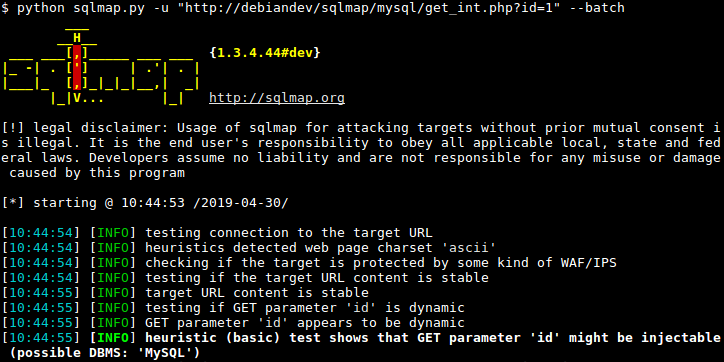
\includegraphics[scale=0.4]{img/sqlmap.png}
    \caption{SQLMap}
    \label{fig:sqlmap}
  \end{figure}

  \item \textbf{suIP.biz:} En principio fue creado para realizar acciones con direcciones IP como pueden ser la recopilacion
  de rangos IP de países, ciudades, etc; obtener información sobre la dirección IP e IPv6, entre otras. Sin embargo, también
  permite realizar pruebas de inyección SQL que está impulsado por sqlmap. Para ello, se debe ingresar la URL de la página
  web a analizar y seleccionar el tipo de inyección SQL a realizar.

  \item \textbf{Acunetix:} Es una herramienta de pruebas de seguridad de aplicaciones que lo ayuda a abordar las vulnerabilidades
  en todos sus activos web críticos. Este escaner de vulnerabilidades es el más maduro del mercado desarrollado desde 2005 en \emph{C++},
  lo que es mucho más rapido que otras soluciones.

  Acuteniz utiliza dos tecnologías únicas que lo ayudan a descubrir más vulnerabilidades: AcuMonitor y AcuSensor. Además, AcuSensor
  le ayuda a encontrar la vulnerabilidad en el código fuente. Además, puede detectar hasta 6500 vulnerabilidades, incluidas las de
  inyección SQL, XSS, CSRF, etc.

  \item \textbf{SQLi Dumper:} Es una herramienta de inyección SQL automática que escanea aplicaciones web en busca de vulnerabilidades de inyección SQL.
  Esta herramienta utiliza un proceso de 6 fases para proporcionar la información solicitada. Cada fase, a su vez, tiene varios pasos:
  \begin{itemize}
    \item Fase 1. Recoger dorks.
    \item Fase 2. Usar un Proxy o VPN.
    \item Fase 3. Insertar dorks e iniciar el escáner.
    \item Fase 4. Haga clic en Inyección SQL e inciar el explotador.
    \item Fase 5. Seleccionar las URL para realizar la búsqueda.
    \item Fase 6. Volcar y guardar los datos.
  \end{itemize}

  Los \emph{Dorks} son criterios de consultas avanzadas para acceder a información oculta.
\end{itemize}


\section{Métodos manuales simples}
Si se está realizando una prueba de penetración de forma manual y se desea verificar la posibilidad de realizar inyecciones SQL,
existen métodos sencillos para llevarlo a cabo.

\begin{itemize}
  \item El primer test consiste en enviar una comilla simple como entrada: 
    '
  Si la entrada es vulnerable, la aplicación generará un error.

  \item El siguiente test implica enviar el siguiente valor:

  \begin{center}
    \begin{BVerbatim}
      '1' and '1' = '1’
    \end{BVerbatim}
  \end{center}

Si la entrada se ejecuta sin problemas, indica que se está inyectando código SQL, ya que la condición '1'='1' siempre es verdadera.

Para verificar, se puede enviar el comando:
\begin{center}
  \begin{BVerbatim}
    '1' and '1' = '0'
  \end{BVerbatim}
\end{center}

Si la entrada NO se ejecuta, se confirma que es posible inyectar código SQL en la entrada, ya que la condición '1'='0' es falsa y, por
lo tanto, el comando no se ejecutará.
\end{itemize}

\section{Ejemplos de casos reales}
\begin{enumerate}
  \item \textbf{Incidente en Heartland Payment Systems (2008)} \\
  En el invierno de 2008, el mundo financiero fue sacudido por un acto delictivo de proporciones digitales. Albert González, un conocido
  pirata informático, lideró un audaz ataque contra Heartland Payment Systems, una empresa encargada de procesar transacciones con tarjetas
  de crédito y débito. A lo largo de varias semanas, el grupo de González utilizó una técnica conocida como inyección SQL para infiltrarse
  en las defensas de Heartland.

  Cada día que pasaba, Heartland se convertía inadvertidamente en un tesoro para González. El ataque resultó en una asombrosa violación que
  afectó a 130 millones de números de tarjetas de crédito y débito. Desde individuos hasta pequeñas empresas, nadie quedó inmune a la magnitud
  de esta brecha, que se extendió por todo Estados Unidos.

  El daño financiero fue abrumador. Heartland enfrentó pérdidas de más de 145 millones de dólares en indemnizaciones por pagos fraudulentos.
  Como respuesta, Heartland reforzó sus protocolos de ciberseguridad, implementando la encriptación de extremo a extremo para proteger los
  datos de las tarjetas, lo que estableció un nuevo estándar en la industria.

  Albert González fue condenado a 20 años de prisión en 2010, marcando el fin de su reinado de terror digital. La brecha en Heartland sirvió
  como un recordatorio contundente de la escala, alcance y potencial devastador de los ataques de inyección SQL.

  \item \textbf{Incidente en Sony Pictures (2011)} \\
  En 2011, un ciberataque envió ondas de choque a través de Hollywood, con Sony Pictures como víctima. El grupo de hackers conocido como LulzSec
  explotó una vulnerabilidad de inyección SQL para infiltrarse en la base de datos de Sony Pictures, dando inicio a una pesadilla digital de varias semanas.

  El impacto del ataque se extendió tan ampliamente como la influencia global de Sony Pictures. Información confidencial se filtró en la red, 
  incluyendo documentos, correos electrónicos e incluso películas no estrenadas. Fue un ataque directo a la industria del entretenimiento, afectando a 
  individuos, empresas y gobiernos asociados con Sony Pictures.

  Las consecuencias fueron significativas. Sony Pictures reportó una pérdida de 15 millones de dólares en su informe fiscal anual, directamente atribuida 
  al ataque. El daño a la reputación de la empresa fue aún más notable.

  Después de que el polvo se asentó, Sony Pictures fortaleció sus medidas de ciberseguridad y estableció estrictas prácticas de seguridad para prevenir 
  futuros desastres. A diferencia de LulzSec, varios de sus miembros enfrentaron consecuencias legales en los años siguientes, subrayando las serias 
  repercusiones legales de la ciberdelincuencia.

  \item \textbf{Brecha en Yahoo! (2012)} \\
  En el verano de 2012, Yahoo!, el gigante digital, sufrió un golpe devastador. El grupo de piratas informáticos conocido como D33Ds Company aprovechó
  una vulnerabilidad de inyección SQL en la base de datos de Yahoo!, obteniendo acceso a una gran cantidad de datos personales.

  Este ataque internacional afectó a aproximadamente 450.000 usuarios de Yahoo! en todo el mundo. Las víctimas abarcaron desde usuarios comunes hasta
  pequeñas y medianas empresas que confiaban en Yahoo! para su comunicación digital diaria. Los datos comprometidos incluyeron nombres de usuario, 
  direcciones de correo electrónico y contraseñas encriptadas de manera insuficiente.

  Las secuelas fueron un testimonio del potencial destructivo de los ataques de inyección SQL. La reputación de Yahoo! se vio afectada y la compañía
  tuvo que enfrentar batallas legales y acuerdos durante años después de la brecha. A pesar de los considerables daños, Yahoo! utilizó esta experiencia
  como catalizador para el cambio. Reforzaron sus medidas de seguridad, introduciendo protecciones más robustas y promoviendo mejores prácticas de contraseñas entre sus usuarios.

  A pesar de que la Compañía D33D no fue identificada, el ataque marcó su punto más alto y también su declive. La comunidad internacional y las fuerzas
  del orden iniciaron una búsqueda que finalmente llevó a la disolución del grupo.

  \item \textbf{Vulnerabilidad en Drupal (2014)} \\
  En octubre de 2014, se detectó una alarma silenciosa en las oficinas de Drupal, un sistema de gestión de contenidos muy popular. Se encontró una
  vulnerabilidad de inyección SQL en su sistema, que podría potencialmente afectar a millones de sitios web en todo el mundo.

  La diversidad de usuarios de Drupal, desde individuos y pequeñas empresas hasta gobiernos y grandes corporaciones, estaban todos dentro del alcance
  de esta ciberamenaza internacional. La naturaleza de los datos en peligro era tan variada como los usuarios de Drupal, desde detalles personales hasta
  datos corporativos sensibles.

  Aunque el daño financiero fue difícil de cuantificar debido a la naturaleza generalizada del ataque, las ondas de choque se sintieron en todo el mundo
  digital. A las siete horas de descubrir la vulnerabilidad, Drupal publicó una actualización de software para corregir el agujero de seguridad. Sin embargo,
  también anunciaron que cualquier sitio no parcheado dentro de esa ventana debía considerarse comprometido, lo que provocó una loca revuelta entre sus usuarios.
    
  A pesar de la ausencia de un autor conocido o de un número preciso de afectados, el incidente de Drupal subrayó el potencial alcance de los ataques de inyección SQL.
  El anonimato de los atacantes fue un escalofriante recordatorio de la naturaleza escurridiza de la ciberdelincuencia. Pero ante la adversidad, la comunidad digital 
  se unió, actualizando sus sistemas y compartiendo medidas defensivas para capear juntos el temporal.

  \item \textbf{Ataque a TalkTalk (2015)} \\
  En otoño de 2015, TalkTalk, un gigante británico de las telecomunicaciones, se encontró en el punto de mira de un despiadado ciberataque. Un grupo de jóvenes piratas
  informáticos, liderados por un adolescente de 17 años, explotó una vulnerabilidad de inyección SQL para burlar las defensas digitales de TalkTalk.

  El ataque se produjo a escala nacional, en todo el Reino Unido. Puso al descubierto los datos personales y financieros de 157.000 clientes de TalkTalk. Números de 
  tarjetas de crédito, datos bancarios, nombres, direcciones, fechas de nacimiento, números de teléfono y direcciones de correo electrónico estaban en juego en este 
  robo masivo de datos.

  Las consecuencias financieras fueron monumentales. TalkTalk declaró unas pérdidas antes de impuestos de 60 millones de libras al año siguiente, consecuencia directa
  del ataque. También se enfrentaron a una multa récord de 400.000 libras de la Oficina del Comisionado de Información por fallos de seguridad.

  A raíz de ello, TalkTalk reforzó sus medidas de seguridad, tranquilizó a sus clientes y trabajó incansablemente para restaurar su empañada reputación. Los jóvenes
  hackers fueron detenidos y se enfrentaron a cargos penales, un severo recordatorio de las graves consecuencias legales de la ciberdelincuencia.

  \item \textbf{Base de Datos de Salud de Estonia (2020)} \\
  En 2020, la pacífica nación del norte de Europa, Estonia, se enfrentó a un ciberataque de una magnitud sin precedentes. A pesar de su reputación de gobierno digital avanzado,
  Estonia no fue inmune a los ataques de inyección SQL.

  El objetivo fue la Base de Datos Central de Salud de Estonia, un tesoro de registros médicos sensibles. Mediante un ataque de inyección SQL, los ciberdelincuentes comprometieron
  potencialmente los historiales médicos de casi todos los ciudadanos de Estonia, una brecha que abarcó toda la nación.
  
  El daño financiero sigue sin revelarse, pero el impacto fue profundo, ya que expuso datos sanitarios privados y sacudió la confianza pública. Este ataque supuso una grave intrusión
  en la privacidad, que afectó tanto a particulares como a entidades gubernamentales.
  
  En respuesta, Estonia emprendió inmediatamente amplias contramedidas, mejorando sus protocolos de ciberseguridad e implantando sistemas avanzados de detección de amenazas para evitar
  ataques similares en el futuro.
  
  Aunque la identidad de los autores sigue siendo desconocida, el incidente envió un duro recordatorio a todo el mundo sobre la importancia de unas medidas de ciberseguridad sólidas para
  salvaguardar la información sensible. La respuesta, la capacidad de recuperación y el compromiso de Estonia con la seguridad digital sirvieron de faro para otras naciones que navegan por
  los procelosos mares de las ciberamenazas.
  
\end{enumerate}

% Nueva página 
\cleardoublepage

\chapter{Buenas prácticas en el diseño de bases de datos para prevenir la inyección SQL}
\section{Introducción a las buenas prácticas}
La seguridad de las bases de datos es un aspecto mas que crítico en el desarrollo de software como ya hemos visto hasta ahora la inyección SQL es una de las amenazas más grandes en este apartado. A modo de resumen ya sabemos que la inyección SQL ocurre cuando un atacante inserta código malicioso “malware” mediante las consultas SQL de una aplicación. Este trocito de código se aprovecha de las vulnerabilidades y compromete la seguridad de la información almacenada dentro de la aplicación. Es por ello que con el objetivo de evitar la inyección SQL, se crearon unos estándares para poder aplicar unas “técnicas” adecuadas para evitar estos problemas. 

Este apartado se centra en explorar y recomendar buenas prácticas específicas que los desarrolladores y administradores de bases de datos pueden adoptar para mitigar los riesgos asociados con la inyección SQL.

De manera general dichas prácticas se pueden dividir en:


\begin{enumerate}
  \item Emplear parámetros en lugar de realizar consultas concatenadas. Estas últimas son conocidas como una de las técnicas más frecuentes para la inserción de código malicioso. 
  La utilización de parámetros previene que el código malicioso sea inyectado en la consulta. Debido a que las consultas concatenadas incluyen directamente variables que pueden 
  tener un contenido malicioso a la hora de hacer la consulta.

  \item Asegurarse de validar todas las entradas de usuario. Este parámetro es crucial para garantizar
  que no se incluye código malicioso. La validación puede lograrse mediante diversas técnicas, incluyendo
  la comprobación del formato, la longitud y el contenido de las entradas.
  
  \item Utiliza filtros de salida para proteger los datos sensibles de posibles exposiciones. Estos
  filtros son eficaces para eliminar caracteres especiales que puedan ser aprovechados para inyectar
  código malicioso.
\end{enumerate}

\section{Consultas concatenadas}
Las consultas concatenadas como hemos dicho anteriormente, al permitir la inyección de código malicioso a
través de la simple concatenación con las entradas de usuario, representan un riesgo evidente, como se 
demuestra en este ejemplo:

\begin{center}
\begin{BVerbatim}
SELECT * FROM users WHERE username = 'admin' AND password = '1234';
\end{BVerbatim}
\end{center}

Un atacante o un “craker” puede llegar a aprovecharlo para inyectar código malicioso y eliminar la tabla
de usuarios de la base de datos.
Para evitar la inyección SQL, resulta de crucial importancia sustituir las consultas concatenadas con el
uso de parámetros. De esta manera, los valores se especifican en la consulta, dificultando la inyección
de código malicioso. Por ejemplo:

\begin{center}
\begin{BVerbatim}
SELECT * FROM users WHERE username = :username AND password = :password;
\end{BVerbatim}
\end{center}

Aquí, la consulta especifica los valores de username y password como parámetros.
\begin{itemize}
  \item La validación de todas las entradas de usuario es un paso esencial para asegurarse de las buenas
  prácticas. También es de debida importancia asegurarse de que las entradas cumplan con formatos específicos,
  limitar la longitud y eliminar caracteres especiales es clave para prevenir la inyección de código malicioso.
  
  \item Los filtros de salida son efectivos para eliminar caracteres especiales, como punto y coma (;), numeral (\#),
  comilla simple ('), comilla doble (“), menor que (<) y mayor que (>), reduciendo el riesgo de inyección SQL.
\end{itemize}


\section{Otras prácticas recomendadas}
Existen otras medidas que se pueden tomar en el diseño de bases de datos para prevenir la inyección SQL y que están dentro de las buenas prácticas para poder 
evitar exploits o funcionamientos inadecuados. Estas medidas son clasificables como las siguientes:
\begin{enumerate}
  \item \textbf{Utilizar tablas separadas para datos sensibles.} Los datos sensibles, como las contraseñas, las tarjetas
  de crédito y los números de seguridad social, deben almacenarse en tablas separadas. Esto dificulta que un atacante 
  acceda a estos datos si logra inyectar código malicioso en la base de datos.

  Los datos sensibles, como las contraseñas, las tarjetas de crédito y los números de seguridad social, deben almacenarse
  en tablas separadas. Esto dificulta que un atacante acceda a estos datos si logra inyectar código malicioso en la base
  de datos.
  
  \item \textbf{Utilizar funciones hash para almacenar contraseñas.} Las contraseñas no deben almacenarse en texto plano en
  la base de datos. En su lugar, deben almacenarse en forma de hash. Esto hace que sea más difícil para un atacante descifrar
  las contraseñas si logra robarlas. Esto se debe a que las tablas hashes están encriptadas por su función hash.

  Las contraseñas no deben almacenarse en texto plano en la base de datos. En su lugar, deben almacenarse en forma de hash.
  Esto hace que sea más difícil para un atacante descifrar las contraseñas si logra robarlas.
  
  Las funciones hash convierten una contraseña en un valor único que es difícil de descifrar. Cuando un usuario inicia sesión,
  la contraseña ingresada se compara con el hash almacenado en la base de datos. Si los hashes coinciden, el usuario se autentica.
  
  \item \textbf{Utilizar procedimientos almacenados.} Los procedimientos almacenados en SQL son conjuntos predefinidos de instrucciones 
  SQL que se almacenan en la base de datos para su reutilización, mejorando el rendimiento, la seguridad y facilitando el mantenimiento 
  de la lógica de la base de datos. Estos procedimientos pueden utilizarse para validar las entradas de usuario y ejecutar consultas SQL
  de forma segura.
  \begin{itemize}
    \item \textbf{Validación de entradas:} Estos procedimientos pueden utilizarse para validar las entradas de usuario antes de ejecutar 
    una consulta SQL. Esto ayuda a garantizar que las entradas no contengan código malicioso.
    
    \item \textbf{Consultas seguras:} También se pueden utilizar para ejecutar consultas SQL de forma segura. Esto ayuda a evitar que un atacante utilice una consulta SQL para inyectar código malicioso en la base de datos
  \end{itemize}

  \item \textbf{Utilizar cifrado para proteger los datos.} Los datos sensibles pueden cifrarse para protegerlos de la exposición.

  El cifrado en el servidor de base de datos se realiza antes de que los datos se almacenen en la base de datos. El cifrado en el cliente se
  realiza antes de que los datos se envíen al servidor de base de datos. El cifrado puede ayudar a proteger los datos sensibles de los ataques
  de inyección SQL. Si un atacante logra inyectar código malicioso en la base de datos, los datos cifrados estarán protegidos.
\end{enumerate}

En conclusión, la inyección SQL representa una amenaza persistente dentro de la seguridad de las bases de datos, con el potencial de comprometer la información de la base. Sin embargo, al adoptar y aplicar rigurosamente las buenas prácticas discutidas en este apartado, los desarrolladores y administradores de bases de datos pueden fortalecer significativamente las defensas de sus aplicaciones contra este tipo de ataques.

Al integrar las prácticas ya comentadas en los procesos de desarrollo y gestión de bases de datos, las organizaciones pueden reducir significativamente las vulnerabilidades ante un ataque de inyección SQL y garantizar un entorno digital más seguro y resistente.

% Nueva página 
\cleardoublepage

% Capitulo 
\chapter{Marco legal y cumplimiento normativo}
\section{Introducción al marco legal}
La inyección SQL como hemos visto hasta ahora, es una gran vulnerabilidad de seguridad en organizaciones o ambientes de desarrollo de software. 
Tenemos que señalar los riesgos provenientes de los ciberataques que han hecho que  la ciberseguridad sea un campo en el que tanto los estados 
cómo las empresas tienen que estar cada vez más pendiente ante el manejo de una gran cantidad de datos en red, mediante ataques informático una
importante cantidad de información confidencial, datos personal son sustraídos a diario. Suponiendo así un gran desafío y un riesgo global.

En un mundo cada vez más interconectado y dependiente de la tecnología, el riesgo a sufrir un ciberataque que destruya o use de manera indebida
la información de carácter personal aumenta exponencialmente. Por ello es de especial relevancia comprender como la ciberseguridad y el cumplimiento
normativo son de gran importancia para asegurar la protección de datos de carácter personal.

La protección de las personas físicas en relación con el tratamiento de datos es un derecho protegido por el artículo 18.4 de la constitución 
española de esta manera nuestra constitución fue pionera en el reconocimiento de la protección de datos de carácter personal cuando dispuso que: 
“la ley limitará el uso de la informática para garantizar el honor y la intimidad personal y familiar de los ciudadanos y el pleno ejercicio de sus derechos”

En el contexto Español, la Ley Orgánica 3/2018, de 5 de diciembre, de Protección de Datos Personales y garantía de los derechos digitales (LOPDGDD), 
con la progresión de esta nueva Ley Orgánica se pretende adaptar el ordenamiento jurídico nacional al reglamento de la Unión Europea 2016/679 del 
Parlamento Europeo y del consejo relativo a la protección de las personas físicas y lo que respecta al tratamiento de sus datos personales y a la 
libre circulación de estos datos. Se establecen las bases legales para abordar la inyección SQL. Dicha ley establece las responsabilidades que deben
de manejar las entidades que influyen o manejan datos personales, para que así estas contengan las medidas de seguridad correspondientes para proteger la información.

Además el artículo 31 de la LOPDGDD registra que aquellos que son responsables del tratamiento de datos deben adoptar medidas necesarias para garantizar
un nivel de seguridad adecuado, incluyendo:

\emph{1. Los responsables y encargados del tratamiento o, en su caso, sus representantes deberán mantener el registro de actividades de tratamiento al que se refiere el 
artículo 30 del Reglamento (UE) 2016/679, salvo que sea de aplicación la excepción prevista en su apartado 5.}
\\ \\
\emph{2. Los sujetos enumerados en el artículo 77.1 de esta ley orgánica harán público un inventario de sus actividades de tratamiento accesible por medios electrónicos
en el que constará la información establecida en el artículo 30 del Reglamento (UE) 2016/679 y su base legal.}

No debemos olvidar que el marco jurídico actual se completa con el Real Decreto 1720/2007 por el que se aprueba el desarrollo de la ley LOPDGDD y el Real Decreto 389/2021 
por el que se aprueba el estatuto de la agencia española de protección de datos.

% Nueva página 
\cleardoublepage

\section{Cumplimiento normativo}
La inyección SQL es una vulnerabilidad de seguridad grave que puede dar lugar a consecuencias penales graves. En España, la Ley Orgánica 3/2018,
de 5 de diciembre, de Protección de Datos Personales y garantía de los derechos digitales (LOPDGDD), establece las siguientes consecuencias penales
para la inyección SQL:
\begin{itemize}
  \item Multa si la infracción se comete por imprudencia grave o negligencia grave.
  \item Prisión de uno a tres años.
\end{itemize}

Además, la inyección SQL también puede dar lugar a consecuencias penales en virtud de otras leyes, como la Ley Orgánica 10/1995, de 23 de noviembre,
del Código Penal. Por ejemplo, la inyección SQL puede utilizarse para cometer los siguientes delitos:
\begin{itemize}
  \item Robo de datos personales (artículo 197.1 del Código Penal).
  \item Daños informáticos (artículo 264 del Código Penal).
  \item Amenazas (artículo 169 del Código Penal).
  \item Coacción (artículo 172 del Código Penal).
\end{itemize}

Por lo tanto, es importante que las organizaciones que manejan datos personales tomen medidas para prevenir la inyección SQL. Estas medidas incluyen:
\begin{itemize}
  \item Implementar controles de seguridad adecuados, como la validación de entrada, el uso de contraseñas seguras y la formación del personal.
  \item Tener un plan de respuesta a incidentes en caso de que se produzca una violación de datos.
\end{itemize}

El Real Decreto 43/2021, de 26 de febrero, por el que se modifica el Reglamento de desarrollo de la Ley Orgánica 3/2018, de 5 de diciembre, de Protección
de Datos Personales y garantía de los derechos digitales:

\begin{center}
  \textbf{“Artículo 28. Obligaciones generales del responsable y encargado del tratamiento.”}
\end{center}
\emph{Los responsables y encargados, teniendo en cuenta los elementos enumerados en los artículos 24 y 25 del Reglamento (UE) 2016/679, determinarán las
medidas técnicas y organizativas apropiadas que deben aplicar a fin de garantizar y acreditar que el tratamiento es conforme con el citado reglamento.}

Establece nuevas obligaciones para las organizaciones que manejan datos personales. Estas obligaciones incluyen:
\begin{itemize}
  \item Implementar medidas de seguridad técnicas y organizativas adecuadas para garantizar la seguridad de los datos personales. Estas medidas deben
  ser proporcionales al riesgo al que están expuestos los datos.

  \item Realizar una evaluación de riesgos para identificar los riesgos a los que están expuestos los datos personales.
  
  \item Seleccionar y aplicar medidas de seguridad adecuadas para mitigar los riesgos identificados.
  
  \item Documentar las medidas de seguridad implementadas.
\end{itemize}

\section{Colaboración con las autoridades}
En el caso de que una organización experimente una intrusión por inyección de SQL, es crucial que ésta colabore con las autoridades para investigar el
incidente. Tenemos que tener presente que cualquier persona física o jurídica tiene un deber de colaboración con las autoridades proporcionando a éstas
la información necesaria para la investigación. Llegar a colaborar con las autoridades puede incluso agilizar el proceso consiguiendo; identificar al atacante,
la recuperación de datos robados y la prevención de futuras intrusiones, aparte de una mayor solvencia en la resolución del problema

Colaborar con las autoridades le proporciona a la organización la oportunidad de aprovechar los recursos y la experiencia de las autoridades en la investigación de incidentes de seguridad. 

Asimismo, las autoridades pueden colaborar en la recuperación de los datos que hayan sido sustraídos durante el ataque, minimizando así el impacto de la intrusión. 
Además, existe la posibilidad que mediante  trabajo en conjunto, la organización y las autoridades puedan llegar a desarrollar estrategias para prevenir futuras
intrusiones al abordar y corregir las vulnerabilidades que permitieron la intrusión inicial.

Enlazado al tópico anterior, existen varios reglamentos que obligan a las organizaciones a colaborar con las autoridades en caso de ciberataques:

La Ley de Enjuiciamiento Criminal, obliga a las organizaciones a informar a las autoridades de cualquier incidente de seguridad que pueda afectar a la integridad
de la administración de justicia.

La Ley de Protección de Datos Personales y garantía de los derechos digitales, que obliga a las organizaciones a notificar a la Agencia Española de Protección de Datos cualquier violación
de datos personales.

El Código Penal, que castiga con penas de prisión los delitos informáticos, entre los que se incluye la intrusión en un sistema informático.

Por todo lo expuesto hemos dejado claro que la inyección SQL presenta un gran reto a las autoridades estatales debido a la vulnerabilidad de seguridad que se puede producir en
las distintas organizaciones o personas físicas y es por ello que todas estas entidades sean capaces de seguir la legislación vigente para poder combatir la inyección SQL.

% Nueva página 
\cleardoublepage

% Capitulo 7
\chapter{Futuro de los ataques de inyección SQL y las bases de datos}
Con el rápido avance de la tecnología, se vislumbra un panorama complejo en la seguridad de sistemas y aplicaciones. Los ataques de inferencia surgen 
como un desafío crítico en el contexto de la Inteligencia Artificial (IA) y el Aprendizaje Automático (Machine Learning, ML).

Los sistemas de ML operan a través de la asimilación progresiva de datos de entrenamiento para perfeccionar sus capacidades de toma de decisiones y 
predicciones. Es bien sabido que cuantos más datos se suministren, mayor será la precisión en las decisiones resultantes. Una vez en producción, 
estos sistemas despliegan sus interfaces de programación de aplicaciones (API) públicas, las cuales son accesibles tanto para usuarios como para 
otras aplicaciones que buscan aprovechar su funcionalidad.
	
Sin embargo, esta apertura no viene sin sus preocupaciones. Los modelos de ML, en muchos casos, operan con datos de una naturaleza extremadamente
confidencial, tales como detalles de tarjetas de crédito o información personal identificable, los cuales representan auténticos tesoros para 
posibles atacantes.

En este contexto, los ataques de inferencia, específicamente los de membresía (MI), emergen como una amenaza latente. En un ataque de este tipo,
el objetivo del atacante radica en obtener los datos subyacentes que sirvieron para el entrenamiento del modelo o incluso comprender su funcionamiento
interno. Estos ataques aprovechan el modo en que los modelos de ML emiten respuestas, basándose en la concordancia entre los datos de entrada y aquellos
utilizados en el proceso de entrenamiento.

La proliferación del Aprendizaje Automático como Servicio (Machine Learning as a Service, MaaS) en los últimos años ha expandido la superficie de ataque.
Empresas que desean implementar modelos sin tener que construirlos desde cero ahora pueden hacerlo mediante servicios en la nube. No obstante, esta comodidad
también implica que los atacantes pueden explotar posibles vulnerabilidades en los modelos de ML, potencialmente llevando a cabo ataques de inferencia contra
múltiples empresas si se descubren fallos en la implementación.

Para abordar estos desafíos emergentes, es crucial reconocer que los ataques a los modelos de IA y ML demandan enfoques de seguridad distintos. No existe un
simple “parche” para solucionar un algoritmo, ya que el problema reside en los datos subyacentes utilizados en el entrenamiento.

Por tanto, se deben implementar controles específicos para mitigar estos riesgos:
\begin{itemize}
  \item Los modelos de ML deben tener la capacidad de generalizar los datos de entrenamiento, asegurando que las puntuaciones sean coherentes entre datos
  previamente vistos y no vistos.

  \item Las API de modelos de ML deben contar con características de limitación para detectar posibles consultas maliciosas, siguiendo el modelo de alerta
  ante múltiples “inicios de sesión fallidos” en una dirección IP, como ejemplo análogo en ciberseguridad.
  
  \item Las pruebas de penetración en modelos de IA y ML deben integrarse como parte fundamental de las actividades regulares de seguridad, desarrollando
  casos de ataque específicos y detallados.
\end{itemize}

% Nueva página
\cleardoublepage

\section{Futuros de las bases de datos}
La migración hacia entornos en la nube se ha establecido como un tema crucial en la gestión de bases de datos en la era actual de la tecnología. Este 
cambio fundamental en la infraestructura de TI ha generado un impacto significativo en la forma en que las organizaciones gestionan y acceden a sus datos.
Figuras influyentes en el ámbito de las bases de datos, como Michael Stonebraker, cuyo legado incluye el desarrollo de PostgreSQL y otras tecnologías vanguardistas,
proporcionan una visión valiosa sobre esta transición hacia la nube.

\textbf{El Rol de la Nube en el Futuro} \\
La afirmación contundente de Stonebraker de que “La Nube está en Tu Futuro” resuena con la estrategia de titanes tecnológicos como Amazon, Google y Microsoft, 
que han invertido recursos sustanciales en el desarrollo de soluciones en la nube. Este movimiento hacia la nube refleja una transformación en la forma en que
las organizaciones abordan el almacenamiento y procesamiento de datos a escala global.

\textbf{Ventajas y Desafíos} \\
La adopción de la nube abre una serie de oportunidades y desafíos para las organizaciones. En el lado positivo, la reducción de costos es un factor determinante. 
Stonebraker destaca que, si bien los precios actuales ya son más asequibles, se espera que la creación de un mayor número de centros de datos y la optimización de
la infraestructura en la nube conduzcan a una reducción aún mayor en los costos de servidores y contenedores.

Además de los beneficios económicos, la elasticidad en el uso de recursos es una ventaja distintiva de la infraestructura en la nube. Las organizaciones pueden
pagar solo por los recursos que utilizan y escalarlos dinámicamente en respuesta a la demanda, lo que ofrece una flexibilidad operativa sin precedentes.

Sin embargo, la transición a la nube no está exenta de desafíos. Consideraciones de seguridad, restricciones geográficas y legales, así como políticas internas de
la organización, requieren una planificación meticulosa. Es fundamental abordar estos aspectos para garantizar una migración exitosa y segura.

\textbf{Estrategias de Implementación} \\
Para maximizar los beneficios de la migración a la nube, Stonebraker subraya la importancia de evitar la dependencia de características propietarias de los proveedores
de servicios en la nube. Se recomienda evaluar opciones como \emph{Platform as a Service} (PaaS), donde se alquila la plataforma y se gestiona la instalación de instancias, o
\emph{Database as a Service} (DBaaS), donde se alquila el uso de la base de datos como servicio.

En cuanto a la selección de instancias en la nube, es crucial considerar cuidadosamente el tamaño y el tipo para satisfacer los requisitos específicos de cada proyecto. Se sugiere 
la posibilidad de iniciar con instancias de gran tamaño y, si es necesario, ajustar dinámicamente los recursos para optimizar el rendimiento.

\textbf{Consideraciones de Rendimiento y Estrategias} \\
Para mejorar el rendimiento en bases de datos alojadas en la nube, Stonebraker propone una serie de estrategias detalladas. Estas incluyen:

Minimizar la interacción humana con la base de datos para evitar posibles errores humanos y garantizar la eficiencia en el acceso a los datos.
Utilizar interfaces basadas en procedimientos almacenados para evitar el uso de cursores, lo que puede resultar en un acceso más eficiente y un procesamiento de datos más rápido.
Modificar la aplicación para evitar la contención de control de concurrencia, lo que puede mejorar la eficiencia en situaciones de alta concurrencia.

Además de estas estrategias, es importante considerar optimizaciones a nivel de implementación del código, como la minimización de modificaciones de datos y la optimización de consultas
para mejorar la eficiencia de la base de datos.

% Nueva página 
\cleardoublepage

% Capitulo 8
\chapter{Estudio sobre un caso real de Inyeccion SQL} 
La seguridad informática, definida como el conjunto de medios y técnicas para proteger sistemas informáticos y los datos que manejan,
juega un papel crucial en el ámbito tecnológico y social. Es fundamental considerar los aspectos de seguridad durante el desarrollo
de software, tanto en contextos profesionales como educativos. En este sentido, se llevaron a cabo pruebas en sistemas web desarrollados
por estudiantes del Instituto Tecnológico de Pachuca para analizar su nivel de seguridad y determinar formas de mejorar la confiabilidad del software.

En este contexto, se abordará la seguridad de los sistemas web desarrollados por estudiantes del Instituto Tecnológico de Pachuca, evaluando su
resistencia ante Inyecciones SQL y determinando la necesidad de reforzar la seguridad durante el proceso de desarrollo.

Las pruebas destinadas a determinar la vulnerabilidad de sistemas web a las inyecciones SQL se llevaron a cabo en aplicaciones desarrolladas por
estudiantes de Ingeniería en Sistemas Computacionales e Ingeniería en Tecnologías de la Información y Comunicación del Instituto Tecnológico
de Pachuca. Estos estudiantes se dividieron en dos grupos de la primera carrera y uno de la segunda, reflejando la proporción de estudiantes en
cada disciplina en el instituto.

Los participantes fueron seleccionados en función de encontrarse en los últimos semestres de sus respectivas carreras, asegurando así que habían
cursado la mayoría de las materias relacionadas con la programación. Esta elección se considera crucial para obtener conclusiones
precisas y representativas, ya que proporciona una visión más realista de cómo se abordan los aspectos de seguridad durante el proceso de desarrollo
de software en el entorno educativo. Las aplicaciones desarrolladas por los estudiantes utilizaron software libre, principalmente PHP como lenguaje de
programación, Apache como servidor web y MySQL como gestor de bases de datos. Dichas aplicaciones presentaron un formulario de inicio de sesión básico
(nombre de usuario y contraseña), cuyo proceso de autenticación se intentó burlar mediante inyecciones SQL.

La primera prueba consistió en una inyección en el campo de texto del nombre de usuario, utilizando 
el siguiente query: 
\begin{center}
  \begin{BVerbatim}
    ‘OR 0 = 0 -- comentario'
  \end{BVerbatim}
\end{center}
\begin{figure}[H]
  \centering
  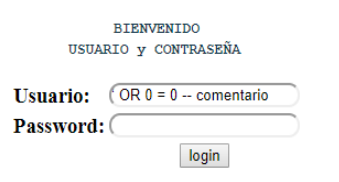
\includegraphics[width=0.5\textwidth]{img/inyeccion_1.png}
  \caption{Inyección en el campo de texto del nombre de usuario}
  \label{fig:inyeccion1}
\end{figure}

% Nueva página
\cleardoublepage

La segunda prueba involucró una inyección en el campo de la contraseña, empleando el siguiente query: 
\begin{center}
  \begin{BVerbatim}
    ‘OR 0 = 0 -- comentario'
  \end{BVerbatim}
\end{center}

\begin{figure}[H]
  \centering
  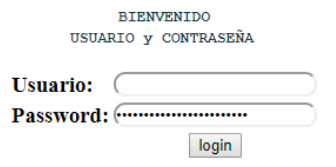
\includegraphics[width=0.4\textwidth]{img/inyeccion_2.png}
  \caption{Inyección en el campo de la contraseña}
  \label{fig:inyeccion2}
\end{figure}

La tercera prueba incluyó la inyección en ambos campos, nombre de usuario y contraseña.
\begin{figure}[H]
  \centering
  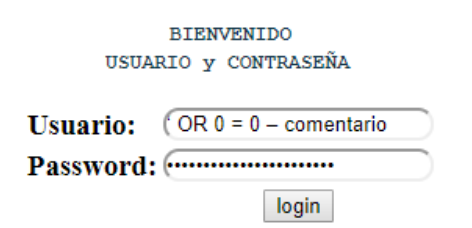
\includegraphics[width=0.4\textwidth]{img/inyeccion_3.png}
  \caption{Inyección en ambos campos}
  \label{fig:inyeccion3}
\end{figure}

Los resultados que se obtuvieron en la prueba de inyección en el campo de inicio de sesión, se vulneraron un total de 13 aplicaciones web. 
De la segunda prueba, la inyección en el campo de la contraseña, resultaron afectadas 19 aplicaciones. Se observa un aumento en el número de aplicaciones 
web vulnerables en la segunda prueba de inyección SQL en el campo de la contraseña, sugiriendo una posible menor protección en comparación con los campos
de texto destinados para el nombre de usuario. Finalmente, de la última prueba, inyección en los campos de inicio de sesión y contraseña, se vulneraron 
6 aplicaciones.En total, se analizaron 81 aplicaciones web bajo las mismas condiciones, de las cuales 38 resultaron vulnerables a las inyecciones. Este 
número representa aproximadamente el 47\% de todos los sistemas evaluados.

Comparación con Estadísticas Generales Según datos del Web Application Security Consortium (WASC), un 12.76\% de las aplicaciones web son vulnerables a inyecciones SQL. 
Al contrastar estas estadísticas generales con los resultados obtenidos en las pruebas, se observa que el nivel de vulnerabilidad de las aplicaciones desarrolladas por 
estudiantes del Instituto Tecnológico de Pachuca es notablemente superior, aproximadamente un 34\% por encima de las estadísticas comerciales. Estos hallazgos refuerzan 
la necesidad de reforzar las medidas de seguridad en las materias relacionadas con el desarrollo de sistemas web.

% Nueva página
\cleardoublepage

Análisis de Códigos y Recomendaciones Examinando los códigos de algunas aplicaciones vulnerables, se identificó que su proceso de autenticación contenía únicamente las siguientes 
líneas de código:
\begin{verbatim}
$usuario = $_POST['usuario']; 
$password = $_POST['password'];
$sql = "SELECT id, id_tipo FROM usuarios 
WHERE usuario= '$usuario' AND password='$password';
\end{verbatim}

Como se mencionó previamente, estas líneas de código son vulnerables durante el proceso de autenticación. Para mejorar la seguridad, se recomendaron modificaciones sencillas a los desarrolladores. En resumen, las siguientes modificaciones fueron aplicadas a sus códigos:

\begin{verbatim}
$usuario = $_POST['usuario'];
$password = $_POST['password']; 
$usuario = mysqli_real_escape_string($mysqli, $_POST['usuario']); 
$password = mysqli_real_escape_string($mysqli, $_POST['password']); 
$sha1_pass = sha1($password);
$sql = "SELECT id, id_tipo FROM usuarios
WHERE usuario= '$usuario' AND password='$sha1_pass'";
\end{verbatim}

Estas modificaciones buscan fortalecer la seguridad de los sistemas y proteger contra futuras inyecciones SQL.

% Nueva página 
\cleardoublepage

% Capitulo 9
\chapter{Bibliografía}

\end{document}